\newcommand{\seccion}{SECUNDARIA INCORPORADA A LA SEG }
\newcommand{\descripcion}{Sumas y restas con fracciones}
\newcommand{\grado}{Primero de secundaria}
\newcommand{\ciclo}{Ciclo escolar: 2015--2016}
\newcommand{\papel}{legalpaper} %letterpaper, legalpaper ...
\newcommand{\fecha}{30 de noviembre de 2015}

\author{M. en C. Reinaldo Zapata}

\documentclass[11pt]{article}
\usepackage[\papel]{geometry}

\title{\flushleft \seccion \\ \descripcion \\  \grado \\ \ciclo}

\newcommand\BackgroundLogo{
\put(162,365){
\parbox[b][\paperheight]{\paperwidth}{%
\vfill
\centering
\includegraphics[width=5cm,height=2.5cm,keepaspectratio]{/Users/reinaldo/Documents/clases/jassa/logo}%
\vfill
}}}

% \hyphenation{con-ti-nua-ci\'on}

\usepackage{enumitem}
\usepackage[T1]{fontenc} %fuentes
\usepackage{lmodern} %fuente mejorada
\usepackage[spanish]{babel}
\decimalpoint
\usepackage{fullpage}
\usepackage{multicol}
\usepackage{graphicx}
\usepackage{eso-pic}
\usepackage{multirow}
\usepackage{subfigure}
\usepackage{tikz}

\begin{document}
\AddToShipoutPicture*{\BackgroundLogo}
\ClearShipoutPicture
\date{\fecha}
\maketitle

A continuaci\'on se presentan una serie de recuadros con sumas y restas de
fracciones. Resuleve cada una de las operaciones.

\begin{figure}[th]
Ejercicio 1: \\
    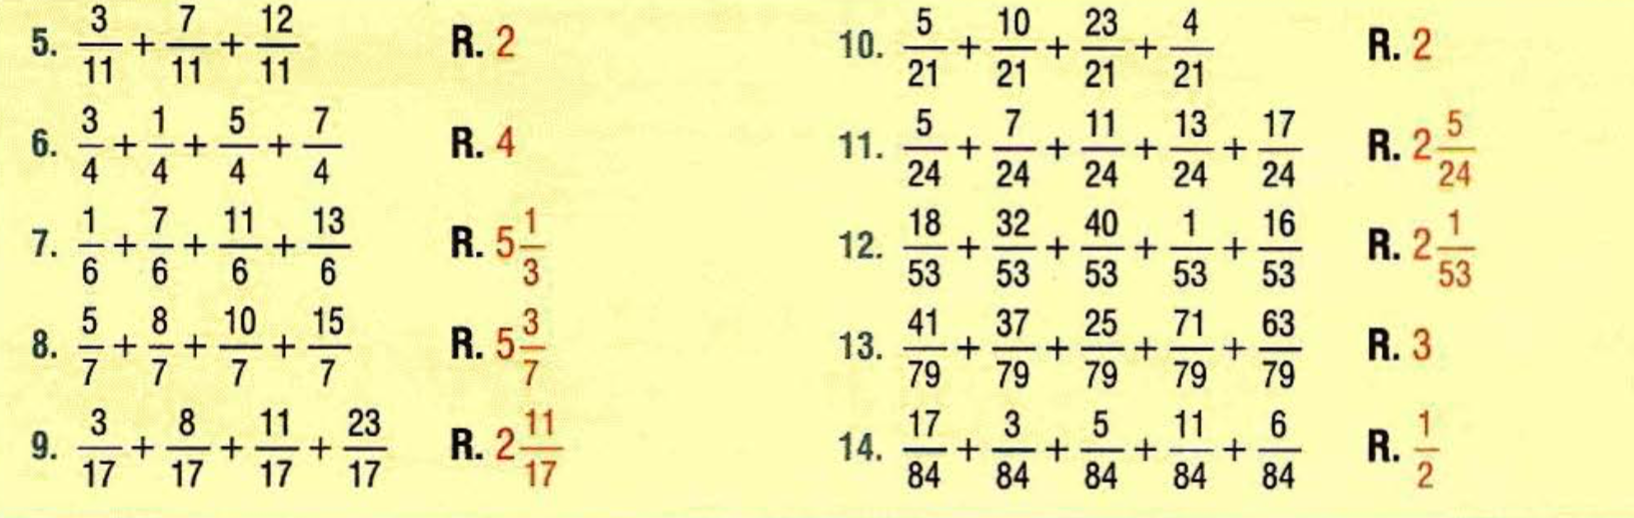
\includegraphics[scale=0.65]{ej1}\\
Ejercicio 2: \\
    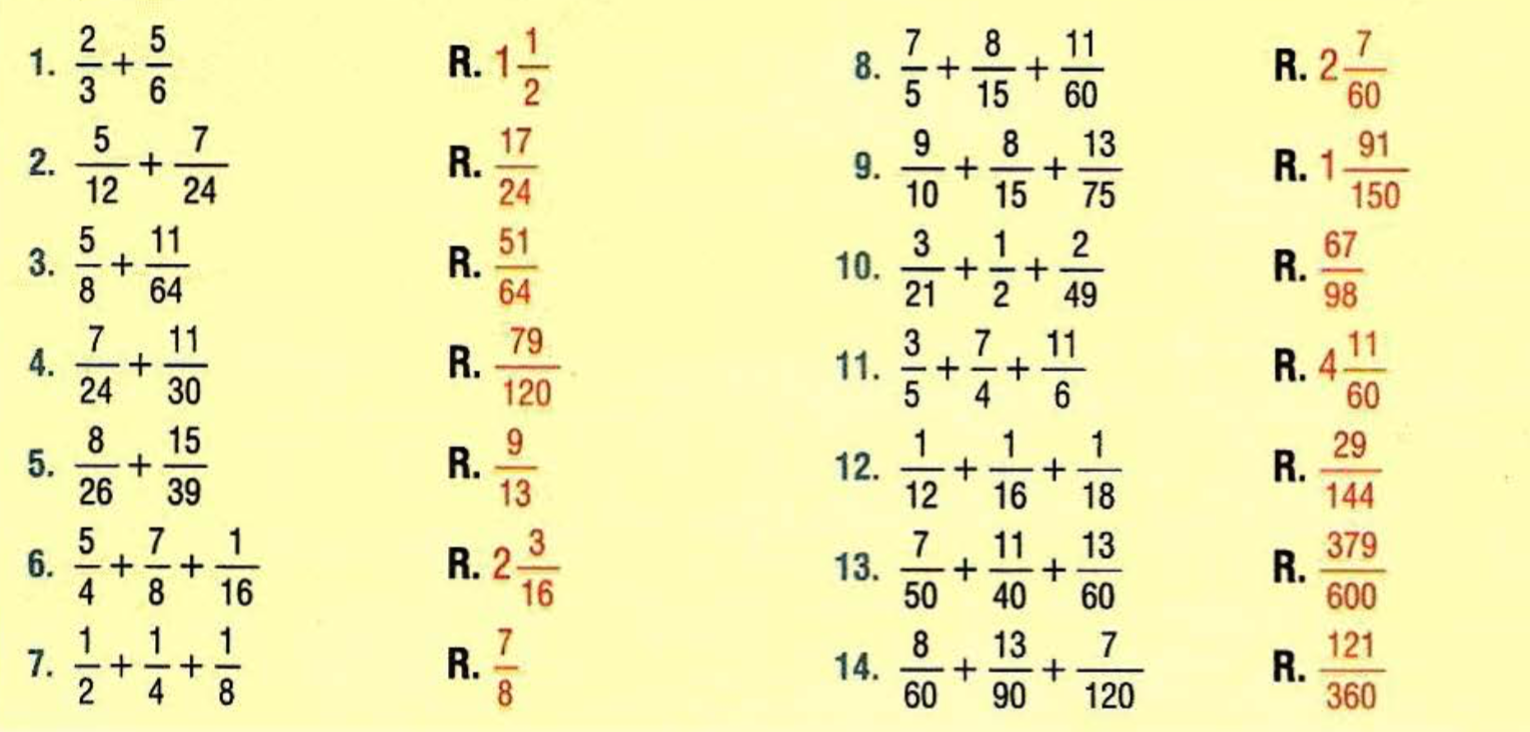
\includegraphics[scale=0.65]{ej2}\\
\end{figure}
    
\begin{figure}[t]
Ejercicio 3: \\
    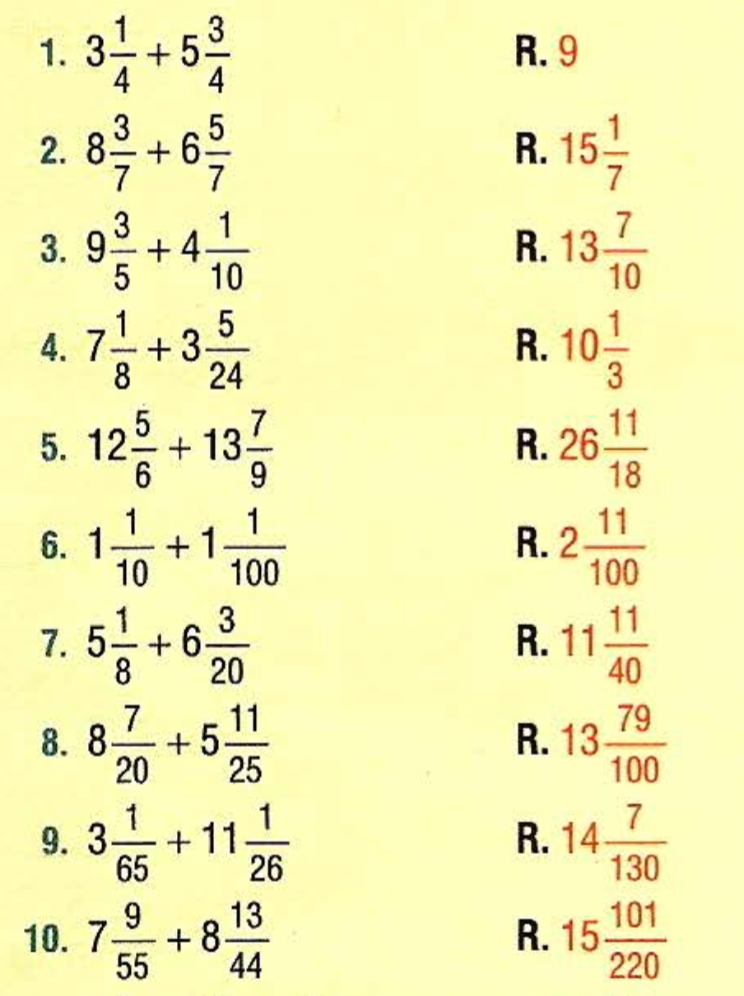
\includegraphics[scale=0.65]{ej3}\\
Ejercicio 4: \\
    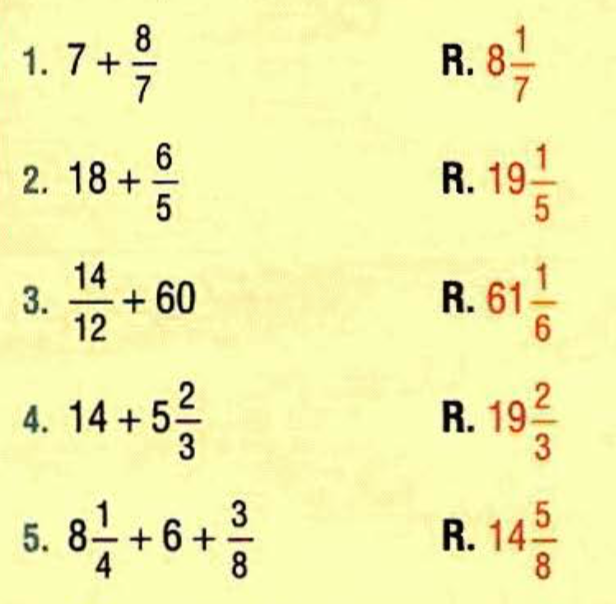
\includegraphics[scale=0.65]{ej4}\\
\end{figure}
    
\begin{figure}[t]
Ejercicio 5: \\
    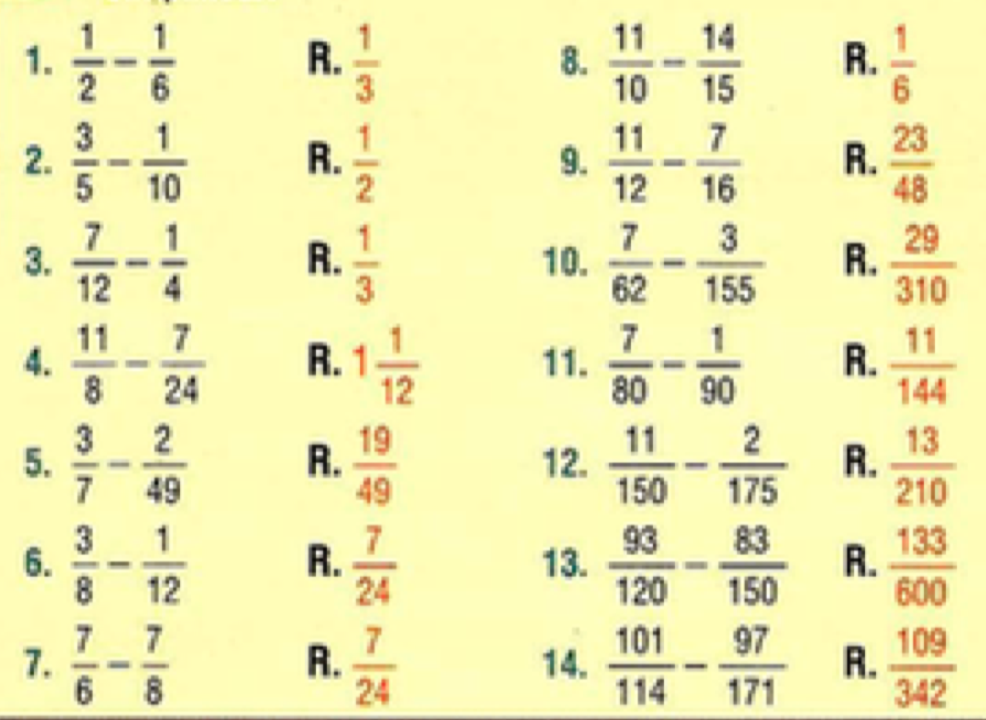
\includegraphics[scale=0.65]{ej5}\\
Ejercicio 6: \\
    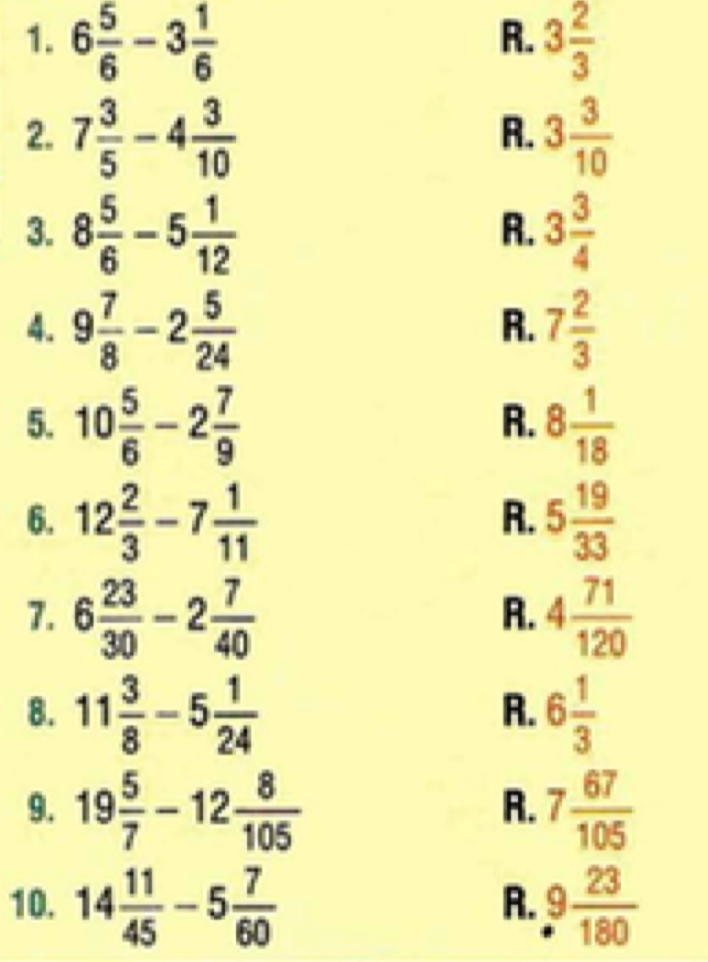
\includegraphics[scale=0.65]{ej6}\\
\end{figure}
    
\begin{figure}[t]

Ejercicio 7: \\
    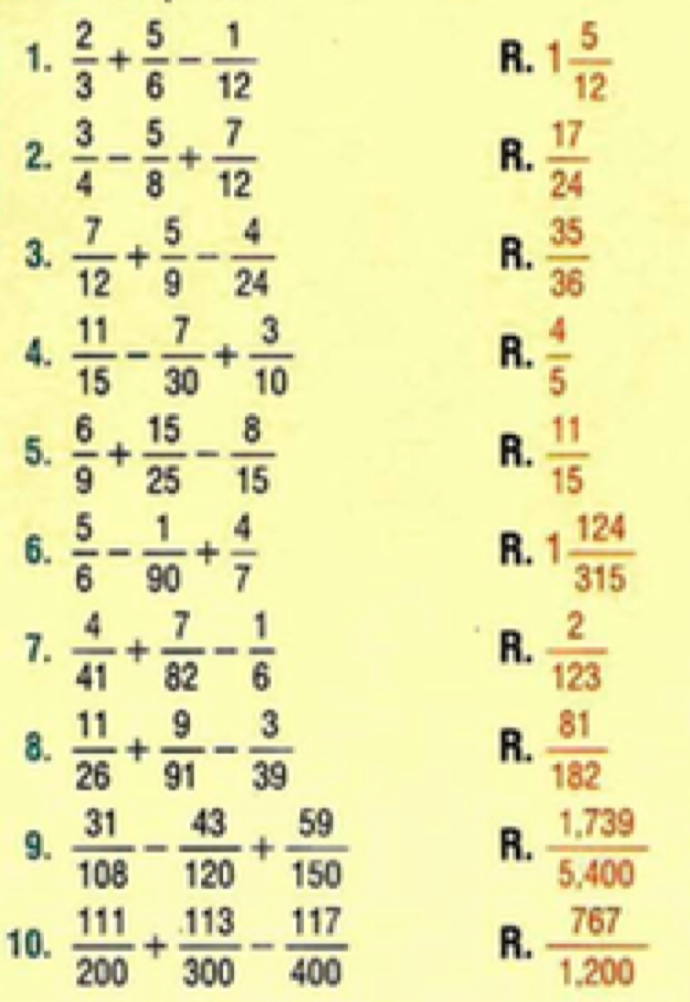
\includegraphics[scale=0.65]{ej7}
\end{figure}


\end{document}






